% Chapter Template
\setstretch{1}
\chapter{Software Design, Industry Engagement, and Hardware Design}\thispagestyle{empty} % Main chapter title
% and Design Research: Community Collaboration in Software Development
\label{Chapter3} % Change X to a consecutive number; for referencing this chapter elsewhere, use \ref{ChapterX}

\lhead{Chapter 3. \emph{Software Design, Industry Engagement, and Hardware Design}} % Change X to a consecutive number; this is for the header on each page - perhaps a shortened title

\setstretch{2}
%-----------------------------------
%	Software Design for Game Jam
%-----------------------------------

\section{Software Design}
A software interface is the part of the software that a person interacts with directly where a software engine is the part of the code that detects and defines what a computer can do with that interaction. 
The interface of software is just as important as the engine, however, because a poorly designed interface will confuse a user, thereby rendering the experience of using the engine potentially opaque. 
screenPerfect's roots are as a software engine, which takes user action and then does things with it. The user interacts with the interface, which speaks to the engine, which then returns values to whichever interface the user has selected.

\newpage
\begin{figure}[h!]
 \centering
 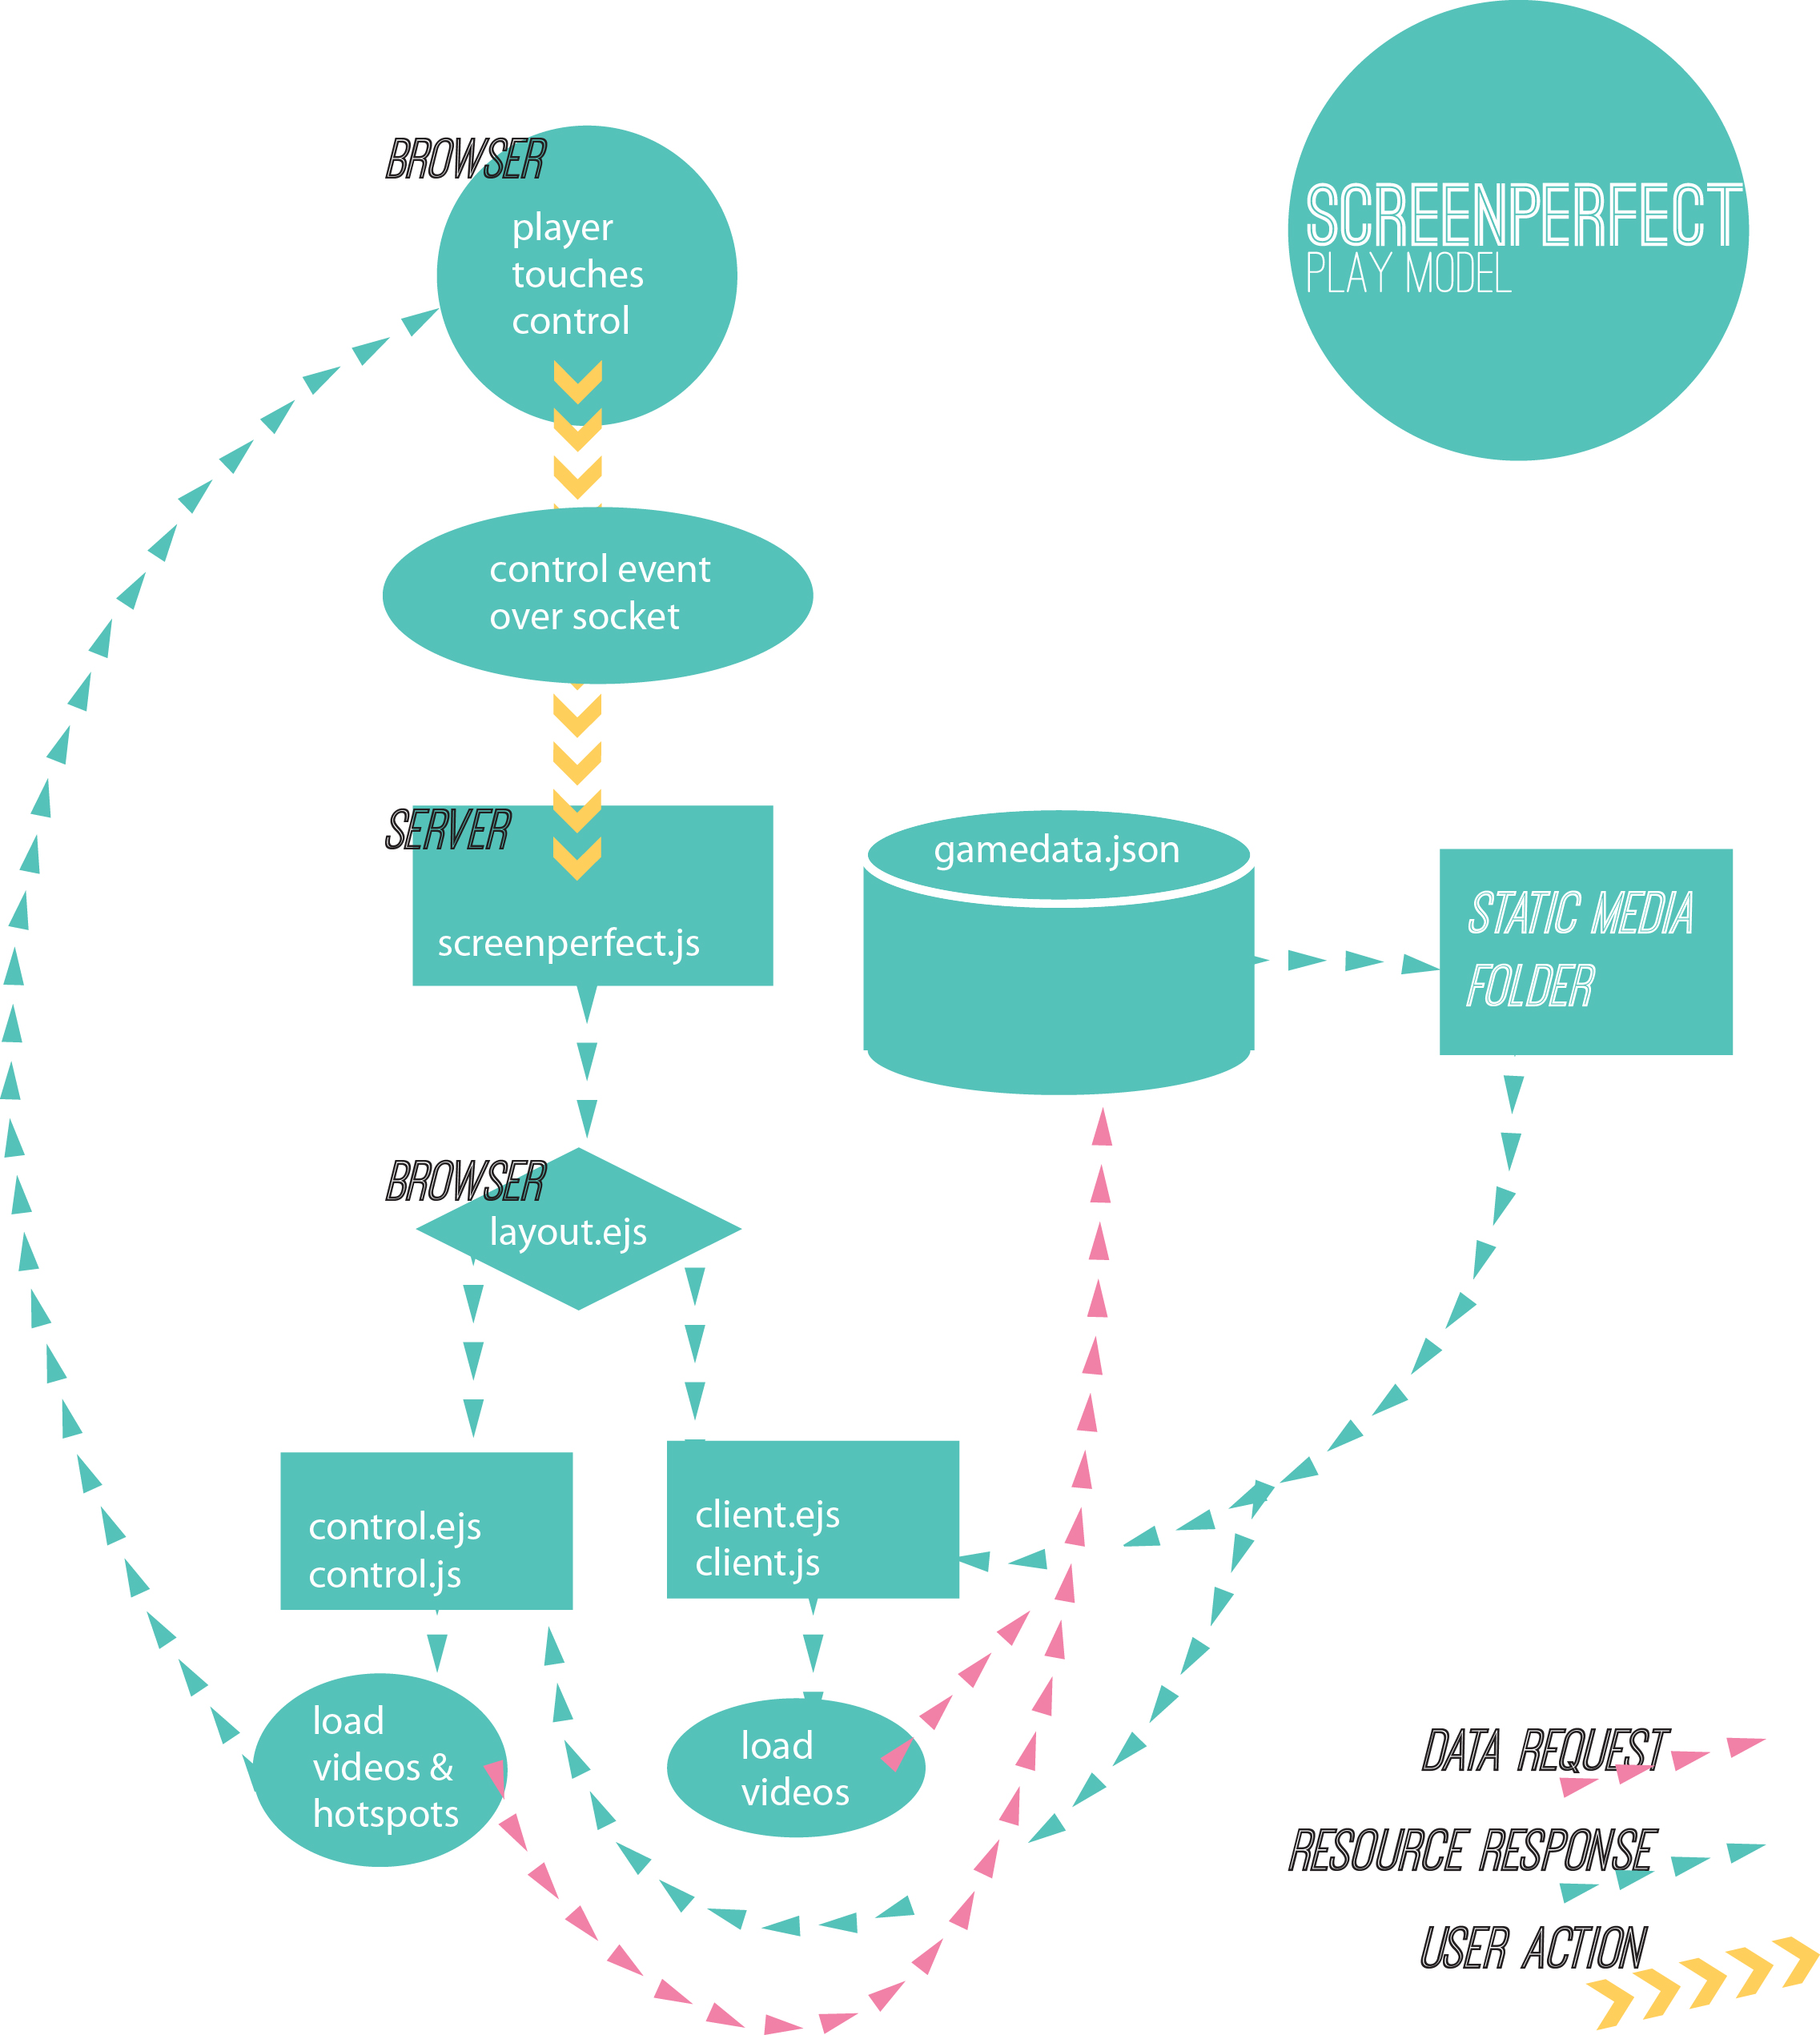
\includegraphics[width=\textwidth]{spCodeFlow}
 \caption{screenPerfect software communication model}
\end{figure}
\newpage

\subsection{screenPerfect Engine|Interface Layout}
In the case of screenPerfect, the interface is laid out in three parts. The first part is the setup screen, which is where game designers load their media (both videos and static files) and lay out the links between those files. This is the essence of a game made in screenPerfect: which choice will a player make to navigate the system as designed by the artist?

The further screens are the client and control screens. screenPerfect supports up to ten client screens and ten control screens, although the interface only exposes a polyphony of client windows, while restricting artists to a single control set for simplicity's sake.

The layout of screenPerfect's editing tools did not work very well for authors who were not already part of the prototyping process. Therefore, as part of the extension of the software for NoJam, Bento Box||Miso reauthored the editing interface of the software. 
The final editing layout is clean, though less expressive than the original design. Rather than hidden tabs, everything is displayed on launch. This permits authors to see their video files during the entire game editing process, which greatly speeds game creation. 
What follows are screencaptures of the pre-fork game jam variant of screenPerfect.

\newpage
\begin{figure}[h]
 \caption{screenPerfect NoJam editor, Asset Population tab.}
 \centering
 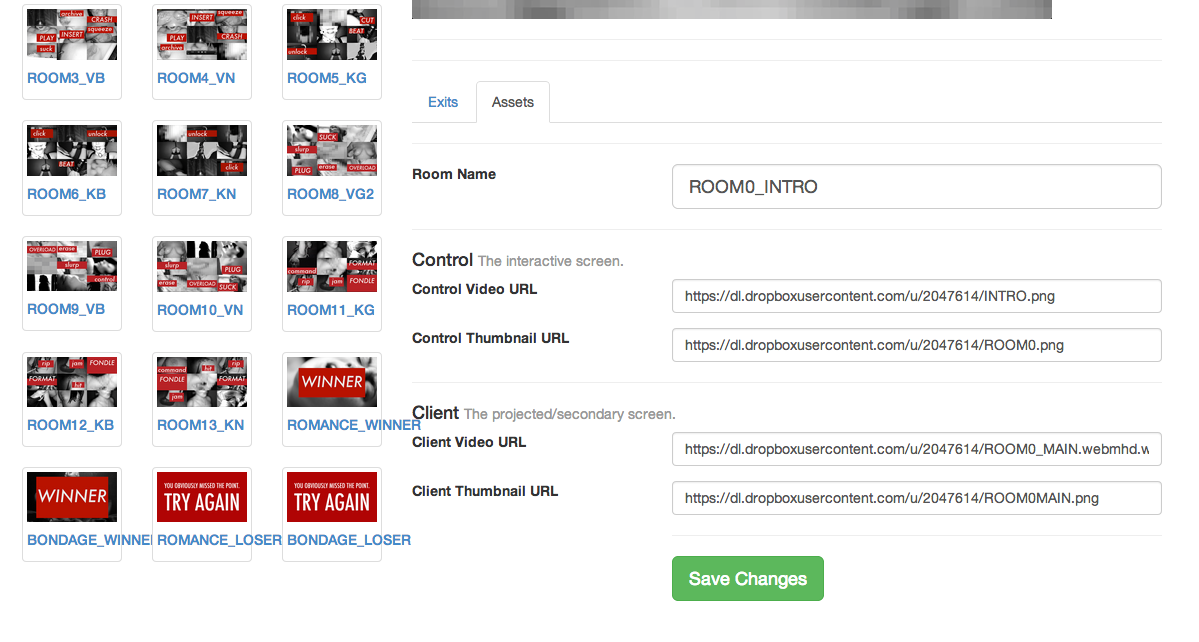
\includegraphics[width=\textwidth]{editSoftAssetTab}
\end{figure}

\begin{figure}[h]
 \caption{screenPerfect NoJam editor, Exit Population tab.}
 \centering
 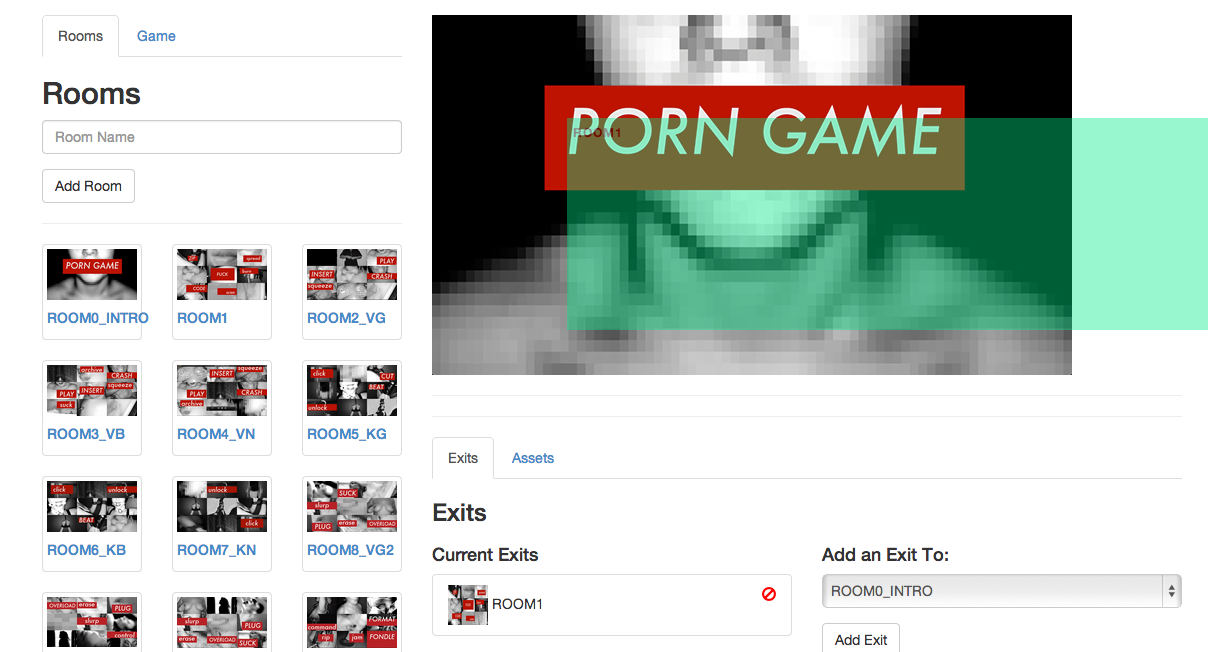
\includegraphics[width=\textwidth]{editSoftExitTab}
\end{figure}

\newpage
%----------------------------------------------------------------------------------------
%	Design Research
%----------------------------------------------------------------------------------------
\section{Design Research}
\subsection{Artist Collaboration}
screenPerfect began with an artistic collaboration, where as a programmer, I worked closely with an artist to reproduce the technical elements of a working practice in order to make it available to other artists in a similar field. This specificity allowed us to develop a very simple tool that solves a minimal set of problems in a tidy fashion. As a developer, it can be difficult to tie work to a given set of problems, or to ensure it has value to an audience outside oneself. Therefore, collaboration gives access to a set of problems that may seem easy 

\section{Development Methods}
\subsection{ Agile Development with an Artist Partner}
The Agile method of software development is based on the Agile manifesto, much as the underlying feminist elements of this project are based on the Cyborg Manifesto, and Cixous' manifesto for the \textit{\'{e}criture f\'{e}minine}. Agile is a response to previous software design practices, called "Waterfall," where software frameworks are laid out and heavily documented in advance of production. Waterfall methods are popular in major software companies, which rely on extensive documentation to communicate between business units. Waterfall emphasizes planning over software production or delivery deadlines. 

The idea of Agile was described in 2001 by a group of software developers \parencite{Agile}. By using an Agile practice of responsive, user-centered design, screenPerfect's interaction model was designed through a series of discussions with key stakeholders, followed by iterative code revisions to a rough first prototype. This can be seen as a hacker-oriented means of development, reflecting Plant's statement that reverse engineering - "starting at the end, and then engaging in a process that simultaneously dismantles the route back to the start" \parencite{plant}. Agile specifically emphasizes individuals and interactions over processes and tools, working software over comprehensive documentation, customer collaboration over contract negotiation, and responding to change over following a plan \parencite{Agile}. 

The screenPerfect development process emerged from a series of linked videos on YouTube, as laid out by Hannah Epstein. We then reviewed strengths and weaknesses of this model: the ability for a large audience with public interlinked video files, but the downside of long load times and ads on pages detracting from the video content. In addition, this required uploading films at low quality to a remote server. From the initial prototype, we asked how the process could be improved, particularly for an exhibition context. 

The game processes laid out in Youtube were converted to a "how might we" - a series of static files presented as interactions in still film. Hannah Epstein laid out an idea of how the video screens should work together, and I confirmed that this system was theoretically possible using websockets - a communication protocol - loaded into a Node.JS application. From there, I wrote a Node app that served basic video files to multiple browser screens simultaneously. This started as a chat application, serving text to three screens simultaneously over websockets. We then replaced the text with video files, layered a control structure over the videos using plaintext JSON files to replace a reliance on a database structure.

A database was not originally required for psXXYborg or later games, because installing a database is an additional step that nontechnical end users cannot be relied upon to find straightforward. Every step of the development process was intended to result in code that is legible to anyone who can read javascript, while being absolutely straightforward to use for a nontechnical video author. 

In development conversations, it became clear that YouTube, in addition to having many distracting advertisements, was very slow to load. This is a problem with reliance on external networks: they cannot be as fast as locally served files. Hannah specifically emphasized speed, smooth loading, and video based in static rather than streaming or live files. These needed to be served within a closed environment to an attentive audience. 

Scripting languages are especially good at this type of development work. I reached out to other developers and asked how they would solve this problem, and they came back to me with a variety of answers - some used PHP, some used Python, all of them relied on JS for their front end. In researching different ways to solve the basic problem - passing a variable back and forth through wireless technology to select two on-screen videos at almost the same time - I discovered the Node.JS software framework, a software package designed to permit developers to use Javascript on both the server and client side of a web application. 

Hannah relied on the h.264 format for her video production, which necessitated an early reliance on the Safari web browser, as HTML5 video does not yet have a settled public codec. Due to conflicts relating to codec patenting, one of many such conflicts that underly the "free" internet, Safari supports H.264 where Chrome supports webm via the V8 engine, the same engine that supports the Node framework. Webm is a compact video format, which results in smaller file sizes and lower bandwidth costs, which eventually affects both load time and playback lag on client machines. 

Overall, Agile worked for this process by allowing a response to user requests for code changes and information rather than forcing work to fit a standard pre-set from above. A waterfall process would have simply not been flexible enough. By working in small steps back from a pre-set destination with total freedom as to how the code actually came together Agile allowed me to demonstrate different working parts of the software as they came together. The documentation for the project is tied into the code commits, and inseparable from the actual written code within its archive.

\subsection{GitHub and Open Source Software}
The development of screenPerfect is dependent on a variety of external technologies. Although relatives and derivatives of Google's V8 system are foremost among these, there is also a dependence on the licencing and mindset of the open-source movement, and the GitHub software repository system.

Open source software is not the same as free software, as provided by structures such as the GNU General Public Licence. Open source is the peer reviewing system of software. Open source means that even if a given piece of software compiles to a single program which can then be distributed for use on the desktop - as screenPerfect does not - the code that goes into the executable file is freely available on the internet, to be changed, supported, and developed by the population of software workers who exist in the broader world. These developers may work on closed or open source projects in their usual working time. They may be very skilled or quite new to development work. What matters is that the software's code is then shared publicly, where it can be reviewed, compiled, extended and changed by anyone at all.

The intent of open source is that anyone may learn from such freely-shared information, and anyone may contribute to the collective knowledge base. There are some obvious problems with open source. One of the clearest is that with intellectual property out there for free, it is a challenge to make any money on an open project. The other is that there is no way to guarantee quality: one takes what one can get, although it is assumed that contributions to projects are made in good faith, and major project contributions are checked by trusted individuals before they are published. For example, the Mozilla project relies on contributors whose code is applied to the codebase after approval by certified reviewers.

\subsection{Licencing}
One of the ways these problems are dealt with is through licensing. The Creative Commons at creativecommons.org expresses their mission as follows: "Creative Commons develops, supports, and stewards legal and technical infrastructure that maximizes digital creativity, sharing, and innovation." It is therefore an appropriate open standard license for creative practice. A preferred license for software development is the MIT Licence, which is closer to the Gnu Public Licence, but does not preclude making money from one's open source work. 

\subsection{Science Fiction Inputs}
My own idea for how this project would work is taken from Cory Doctorow's Pirate Cinema, which features a scene wherein characters climb trees, and using pico projectors already built into their phones, assemble a movie theatre from nothing more than sheets and ropes in the trees \parencite{doctorow}. I felt this sort of mesh-networked sharing is much more likely than a continued reliance on the surveilled internet for sharing copyrighted and copyrighted- material derived works. Since I could not find a system that would permit this type of sharing on the internet, I felt that this project would provide a good chance to build one.
 
\section{Industry Engagement}
\subsection{Game Jams, A Design Method}
A game jam is a variant on the hackathon, which is a type of prolonged effort at taking an idea from concept to finished product in a limited period of time. Game jams are related to design charettes or parallel prototyping \parencite{martin}(Martin, 2012), a method whereby participants rapidly prototype a design idea over a short, intense period of time. A jam - or hackathon - gives registered participants a common area and space to set up their own supplies, and a theme. The group members come to the event with an idea and possibly some resources - video files, sound capability and so on - and use the jam time to assemble a game.

Generally, a game jam will produce a panoply of small game ideas with fleshed mechanics but simple art and sound design in order to demonstrate a possible path forward for a device or piece of software, which will then be polished at a later date, and presented to the indie community either online or at a social event. Sometimes these works will then go on to be finished commercial products, or are intended for further consumption at major conferences such as Indiecade or GDC. These conferences can further the careers of the developers by providing access to funding bodies: publishing houses, or in Ontario, the Ontario Media Development Corporation. Other funding sources can include research groups, such as the SSHRC. By classing game jam development as research, participants released from the need to make commercially appealing works. In the case of Dames Making Games and screenPerfect, funding came from the Feminists in Games project, headed by Jen Jenson of York University, and GRAND FRAGG, a research project dedicated to expanding the diversity of voices represented in gaming. 

Game jams can be time consuming to prepare, as they involve a great deal of communication on the part of the organizers. In order to run a jam, one must open the application period well enough in advance to ensure a large cohort of skilled users who are likely to be interested in producing content with the available tools, or interested in exploring new tools on offer. Typically, jam attendees have a theme suggested - "Mother May I" or "Snacktember" being a few run in 2013 by the Dames Making Games - and then participants bring their own preferred technology to produce a fast prototype over a weekend.

\subsection{Dames Making Games and Game Jams}
\begin{quote}
Dames Making Games (or DMG Toronto) is a non-profit community organization based in Toronto dedicated to supporting dames interested in making, playing, and changing games. In short, we want to build an \textbf{inclusive} and \textbf{engaged} local community of game-makers. Our community isn't women only, but it is women-driven.
\textit{from the DMG.to website, accessed November 27, 2013}
\end{quote}
The Dames Making Games are a community group in Toronto that work to promote women in video games. They have been funded in part by FiG (\url{http://www.feministsingames.com}) and in part by member donations. I am an original director and advising director with the organization, which has given me ready access to a test audience for my ideas with regards to development tools. The Dames Making Games use the game jam method to introduce women and allies to simple game development tools. This provides a straightforward introduction to concepts of computer logic and programming for some people, to video game art development for others, and video game sound production for still others. Some develop system mechanics, some design whole levels or game narratives. 

The point of the DMG is to promote access to this field to people other than the 18-to-35 year old males who form the primary demographic for the video game industry \parencite{igda}\parencite{esa}, in the hopes that a diverse population of game makers will produce a diverse population of games.

The Dames Making Games are interested in screenPerfect as it provides an underlying template for a game-making system that might be easier for newcomers to use than other freely available game engines. The other two members of the Board of Directors of DMG are Cecily Carver and Jennie Faber, who, in exchange for development work as members of Bento Box, have since forked screenPerfect to become a more elaborate engine, called iV in honour of the idea of a Twine engine that created branched narratives from Vine videos \parencite{klimas}.
\subsection{Bento Miso and Bento Box}
Game jams require both space and people who are interested in working on games. A themed game jam, such as No Jam 2, which was designed to test specific software, requires a specific audience and support. In order to access that space, I worked with the Bento Miso co-working facility here in Toronto, with OCADu's game:play lab and Emma Westecott, and with Bento Box, a development company that runs Bento Miso as a not for profit co-working facility.

Miso is a not-for-profit community coworking facility that serves as home for both Bento Box, a local development hub, and the Dames Making Games. It is also the hub of a great deal of Toronto's independent game development community. Miso/Bento Box offer professional support and development advice to game developers, and I felt there was a good match between their professional skillset and my research interests. The Dames Making Games group regularly run a jam in November, and felt that screenPerfect - a new software designed to be accessible in a short time frame to people with extant skills - would be a good match for the audience associated with the organization. 

Bento Box was also at the time seeking an engine that could display the capabilities of their private computer language, Daimio, which offers users the ability to reprogram work on the fly in the browser without being a trusted network source. Therefore, I accepted their help and their offer of hosting the jam in return for giving them permission to fork - copy, reproduce, and extend - my engine under their name. 

Miso, and Bento Box, offered to help me with coding a more accessible front end to the screenPerfect engine in time for the jam, so that I could get feedback on the system mechanics rather than just the interface. 

\subsection{NoJam 2: Video Video}
DMG have a great deal of experience running jams, and therefore, I partnered with DMG/Miso to access to a group of skilled animators, filmmakers, and gamemakers. By partnering with them, I gained ready access to their community population, and they gained access to my software. One of the most common difficulties with game jams is that the short timeframe can cause a lot of frustration to new non-programmers: they spend a lot of time wrestling with tools, rather than generating the content of their games. The DMG would like to make it more straightforward for their membership to generate games and interactive narratives in a short period of time.

No Jam is a two-week jam scheduled by the DMG in November. In order to prepare screenPerfect for the jam, I handed over the basic engine to Bento Box - the production arm of Miso - who cleaned the interface elements and released a web-based version of the software for users. This was a win for them, as they were able to refactor my local code base to take advantage of a new language they have produced, called Daimio. Daimio, being a dataflow language, is ideal for describing choice patterns as they relate to a database. ScreenPerfect is a good engine match for types of games that rely on interactive choices.

As a pair, Dann Toliver - architect of Daimio - and I worked together to clean up the javascript elements of screenPerfect for speaking to the Daimio dataflow language. The group then released a refactored version of the code in time for No Jam, so that our participants could get a clean version of the software to work with. This was challenging for me, as it involved a great deal of trust, and moved the software away from how I had initially envisioned the UI. In particular, we needed to scrap an early idea for a branched narrative "tree" display, which was not included, although it had been planned all along.

After we received No Jam applications, we went through to choose participants who seemed interested the theme and the software restrictions, sent out acceptances, ordered food, and generally set the dates. Applicants were provided diaries to record their working process over the course of the week. The first weekend of the jam consisted of workshops from a variety of specialists to provide direction in how to think about the software and the jam process as research. My presentation is included in Appendix C, consisting of how to work with the screenPerfect software, how to think about multi- screen video, and how to think about technology as a form of creative practice.

The applicants were then sent home for a week to work on their video projects, and asked to document their ongoing process with one another on a private Google Group. Most participants ignored this request, which left us with relatively little online material.

On the actual weekend, we asked that participants arrive with the majority of their video content and design prepared. There were uneven responses to this request, which strongly affected the ability of participants to produce a finished game by the end of the weekend. I interviewed each group early in the process, and then later polled them with informal questions regarding their experience with the software. 

The group experience with the software proved interesting. Accomplished filmmakers had a better time with it, but the most surprising response was from young, self-identified gamemakers, who rather than exploring what was possible within the context of the software tools, decided instead to try to use them to reproduce existing game types, many of which were totally incompatible with the software's design. Of particular interest was the group who tried to reproduce a classic Japanese roleplaying game within the context of video: this did not work so well, and they continued to work at it even after it became apparent it was unlikely to go well. The game itself remains unfinished, but deserves mention as the most unique and possibly stubborn effort. Used to working with uncooperative tools, the participants seemed unsure how to cooperate with a tool clearly designed to a single end. 

Despite this, No Jam was a success, with nine groups producing diverse works on ideas such as how to express a practice of mindfulness, how to work with pornography in a way that forces the viewer to interact with what's happening on screen, exploring systematic violence against women, exploring narratives of imprisonment, magic, and in one unique case, permitting a puppet to escape a toy box. 

In setting up No Jam, we did present at least one workshop on the importance of the personal narrative in producing creative work, which may have influenced the results. Game jammers mostly described their interest in producing work that was finished, and one jammer explicitly stated that she was pleased to have had a finished work at the end of the jam, this being an uncommon result for her when she had to learn the usual round of new software each time. No Jam resulted in at least five "finished" works, which have since been included in several exhibitions around the city, including the December and January Toronto Long Winter series.